\chapter{Background Suppression}\label{sec:background-suppression}

This chapter shows the procedure in suppressing various kinds of backgrounds by applying cuts on MVA classifier outputs. More information about the MVA training, feature importance and hyper-parameter optimization for each MVA step in this chapter can be found in the Appendix \ref{sec:mva-control-plots}.

\section{Resonant Background}
\label{sec:res_bkg}

In this analysis we study decays with kaons in the final state. This means that standard procedures in $b \to u$ analyses in order to suppress $b \to c$ backgrounds, such as $K$-veto, are not possible. As a consequence, our final sample consists of combinations of $K$ pairs coming also from $b \to c$  sources, such as $D^0 \to K^+ K^-$. Such candidates usually have resonance-like properties in the two-kaon invariant mass spectrum. Figure \ref{fig:res_bkg} shows this invariant mass spectrum of two kaons, $m_{KK}$, where obvious resonant structures are present from sources like
\begin{itemize}
	\item $\phi \to K^+K^-$ (sharp resonance at $\sim1.019\e{GeV}/c^2$),
	\item $D^0 \to K^+K^-$ (sharp peak at $\sim 1.864\e{GeV}/c^2$),
	\item $D^0 \to K^+ \pi^-$ (wide, shifted peak, due to kaon miss-identification).
\end{itemize}

In order to suppress these resonant backgrounds, while studying signal or control decay, we impose a set of the following cuts
\begin{itemize}
	\item Signal cut: $\vert m_{KK} - m_{\phi} \vert > \Delta_\phi$, $\vert m_{KK} - m_{D^0} \vert > \Delta_{D^0}$, $\vert m_{K\pi} - m_{D^0} \vert > \Delta_{D^0}$,
	\item Control cut: $\vert m_{KK} - m_{D^0} \vert \leq \Delta_{D^0}$, $\vert m_{K\pi} - m_{D^0} \vert > \Delta_{D^0}$,
\end{itemize}

where $m_{KK}$ is the $KK$ invariant mass and $m_{K\pi}$ is the invariant mass of $KK$, where the kaon's mass, which has the same charge as the $B$ meson, was given the mass of the $\pi^0$ particle, and where $m_\phi \approx 1.019\e{GeV}/c^2$ and $m_{D^0} \approx 1.864\e{GeV}/c^2$ are nominal masses of the $\phi$ and $D^0$ mesons, and $\Delta_\phi \approx 8\E{-3}\e{GeV}/c^2$ and $\Delta_{D^0} \approx 1.5\E{-2}\e{GeV}/c^2$ are symmetric cut widths around the nominal mass values for the $\phi$ and $D^0$ mesons, respectively. By imposing the signal or control cut on our data, we are able to efficiently isolate the desired subset, which is very useful for further studies of the control decay. Table \ref{tab:cut_eff} shows the subsample efficiency after applying either of the cuts.

\begin{table}[H]
	\centering
	\begin{tabular}{l|c|c|c}
		& $\epsilon$(Signal cand.)& $\epsilon$(Control cand.) & $\epsilon$($\phi$ resonance cand.)\\
		\toprule
		Signal cut & $95.4\%$ & $4.0\%$ & $13.6\%$ \\
		Control cut & $1.9\%$ & $96.0\%$ & $0.0\%$ \\
		\bottomrule
	\end{tabular}
	\caption{Various subset efficiencies after imposing the signal or control cut on the $KK$ invariant mass.}
	\label{tab:cut_eff}
\end{table}


\begin{figure}[H]
	\centering
	\captionsetup{width=0.8\linewidth}
	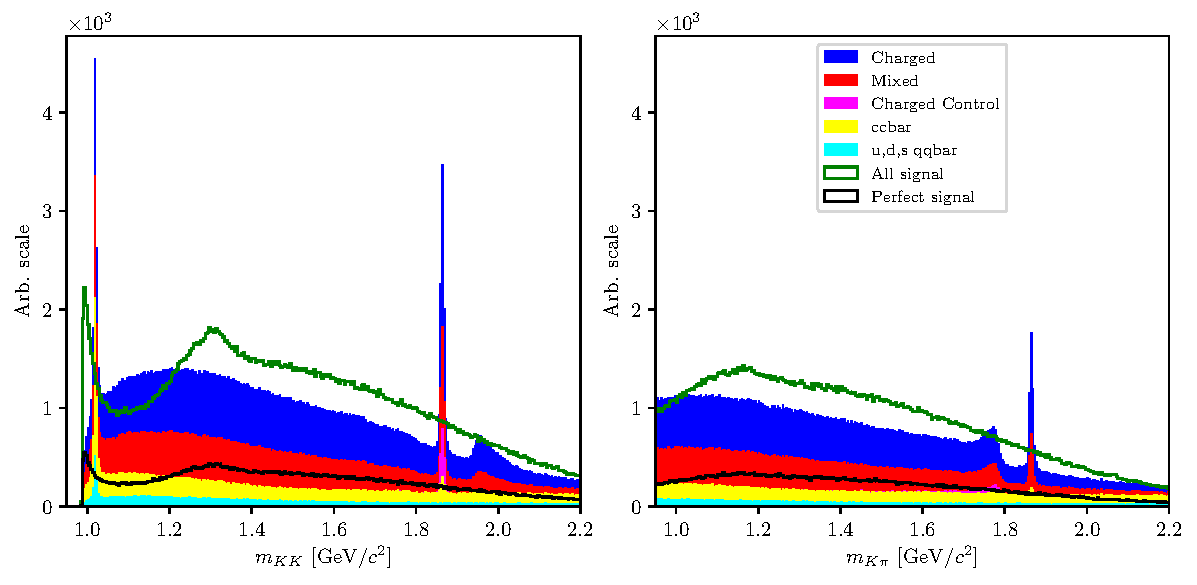
\includegraphics[width=\linewidth]{fig/res_bkg}
	\caption{Invariant mass of two correctly reconstructed kaons (left) and invariant mass of two kaons, where one was miss-identified as a pion (right). Signal (green) and perfect signal (black) are equally scaled up.}
	\label{fig:res_bkg}
\end{figure}


\section{Continuum Suppression}

Continuum background are physics processes where continuum states are produced in electron and positron collisions $$e^+ e^- \to q \bar q,$$ 
where $q = u,~d,~s$ or $c$, and are a sizable contribution to $B \bar B$ events. Additionally to kinematic constraints to separate $e^+ e^- \to \Upsilon(4S) \to B \bar B$ decays from $e^+ e^- \to q \bar q$, properties of the "event shape" are also often used, because phase-space distributions of decayed particles differ for these two processes. Continuum background events are generated in a back-to-back way in the CMS frame, so hadrons produced in the quark fragmentation possess only a small transverse momentum compared to the initial momentum magnitude. This leads to a spatially confined, jet-like structure. On the other hand, $B$ mesons from $B \bar B$ events are produced almost at rest in the CMS frame. Their decay products form an isotropic distribution in the detector, which yields a spherical event shape.

\subsection{Characteristic Variables}
\label{ss:charvar}
Information on the phase-space distribution of decay particles is obtained in a number of different ways. In this subsection different characteristic variables are presented which are used in the MVA training. They all focus on kinematic and shape differences between the two processes, which we want to discriminate. 

%\subsubsection{$B$ meson direction}
%Two $B$ mesons, coming from a spin-1 $\Upsilon(4S)$ meson, both have 0 spin, which results in a $\sin^2\theta_B$ angular distribution of the $B$ meson direction with respect to the beam axis. On the other hand, $q \bar q$ final states are represented by two half-spin fermions, which results in two jets, following a $1+\cos^2\theta_B$ distribution. The variable $\vert \cos \theta_B \vert$ allows one to discriminate between $B$ candidates from $B \bar B$ decays and continuum background. Figure X shows the distribution of $\vert \cos \theta_B \vert$ for different $B$ meson candidates.

\subsubsection{Thrust and Related Variables}
It is possible to define a thrust axis $\vec{T}$ for a collection of $N$ momenta $p_i$ as a unit vector along which their total projection is maximal. Thrust axis $\vec T$ can be obtained by maximizing the expression
\begin{equation}
\vec{T} = \frac{\sum_{i}\vert \vec{T} \cdot \vec{p}_i\vert}{\sum_{i}\vert \vec{p}_i\vert}.
\end{equation}
In this case, a related variable is $\vert \cos\theta_T\vert$, where $\theta_T$ is the angle between the thrust axis of the momenta from $B$ meson decay particles and the thrust axis of all particles in the ROE. Since both $B$ mesons in $B \bar B$ events are produced at rest, their decay particles, and consequentially their thrust axes, are uniformly distributed in the range $[0,~1]$. On the other hand, decay particles from continuum events follow the direction of the jets in the event. As a consequence, the thrusts of both the $B$ meson and the ROE are strongly directional and collimated, which results in a large peak at $\vert \cos\theta_T\vert \approx 1$. Additionally, one can also use the variable $\vert \cos\theta_{TB}\vert $, which is the thrust axis between the $B$ candidate and the beam axis. For $B$ candidates from $B \bar B$ events, this distributions is again uniformly distributed, while for candidates from continuum events this distribution follows the distribution of the jets with the function $1+\cos^2\theta_{T,B}$. Practically, such a distribution exhibits a drop at $\vert \cos\theta_{TB}\vert \approx 1$, due to the acceptance loss of the detector in the direction of the beam pipes. Figure \ref{fig:cosplots} shows the distributions of $\vert \cos\theta_T\vert$ (left) and $\vert \cos\theta_{T,B}\vert$ (right) for different $B$ meson candidates.

\begin{figure}[H]
	\centering
	\captionsetup{width=0.8\linewidth}
	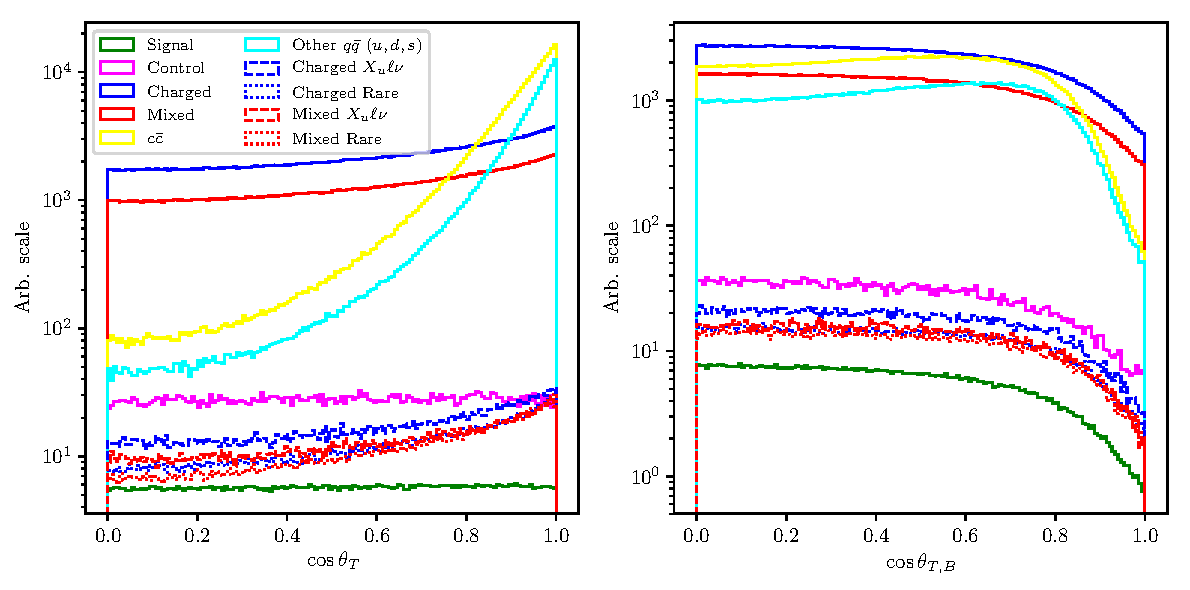
\includegraphics[width=\linewidth]{fig/cs_cosplots}
	\caption{Distributions of $\vert \cos\theta_T\vert$ (left) and $\vert \cos\theta_{T,B}\vert$ (right) for different $B$ meson candidates.}
	\label{fig:cosplots}
\end{figure}

\subsubsection{CLEO Cones}
CLEO cones have been introduced by the CLEO collaboration \cite{asner1996search} and are an additional specific tool to provide optimal background discrimination. They are nine variables corresponding to the momentum flow around the thrust axis of the $B$ meson candidate, binned in nine cones of $10^\circ$ around the thrust axis, as illustrated in Figure \ref{fig:ccones}. 

\begin{figure}[H]
	\centering
	\captionsetup{width=0.8\linewidth}
	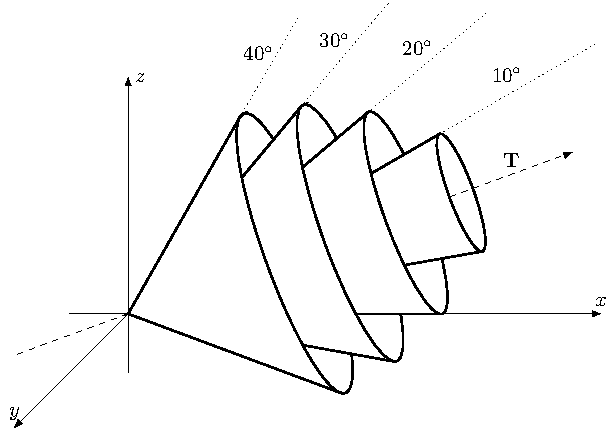
\includegraphics[scale=1]{texfig/CCones}
	\caption{Concept of CLEO cones. $\vec{T}$ denotes the thrust axis of the $B$ meson candidates in the event. Each variable corresponds to a momentum flow around the thrust axis in steps of $10^\circ$.}
	\label{fig:ccones}
\end{figure}

\subsubsection{KSFW Moments}
Fox-Wolfram moments are another useful parametrization of phase-space distribution of energy flow and momentum in an event. For a collection of $N$ momenta $p_i$, the $k$-th order normalized Fox-Wolfram moment $R_k$ is defined as
\begin{equation}
R_k = \frac{H_k}{H_0} = \frac{1}{H_0} \sum_{i,j} \vert p_i \vert \vert p_j \vert P_k(\cos \theta_{ij}),
\end{equation}
where $\theta_{ij}$ is the angle between $p_i$ and $p_j$, and $P_k$ is the $k$-th order Legendre polynomial. For events with two strongly collimated jets, $R_k$ takes values close to 0 (1) for odd (even) values of $k$, so these moments provide a convenient discrimination between $B \bar B$ and continuum events.

Belle developed a refined generation of Fox-Wolfram moments, called Kakuno-Super-Fox-Wolfram (KSFW) moments to further suppress the continuum background. There are $17$  different KSFW moments which are grouped into $R^{so}_k$, $R^{oo}_k$ and $R^{ss}_k$ \cite{bevan2014physics}. The latter ones are excluded due to correlations with $B$ meson specific variables.

\subsection{MVA Training}
\label{ss:qqmva}
Most of the characteristic variables, described in section \ref{ss:charvar}, were taken together in order to train a single MVA classifier for continuum suppression. All characteristic variables were checked for possible $q^2$, $M_{BC}$ or $\Delta E$ correlation. Variables with significant correlation or complex shapes in the correlation distribution were discarded from the training set, since they would have introduced unwanted dependence on the unreliable model, ISGW2, used for signal MC generation. Additionally, all of the characteristic variables in our set do not depend on the signal mode, they only differ in the kinematic and topological aspects of $B \bar B$ and continuum background events.

The training dataset consisted of $2\E5$ candidates, where $50~\%$ of the candidates are correctly reconstructed signal events, $25~\%$ are $u \bar u$, $d \bar d$ and $s \bar s$ background with expected proportions, and $25~\%$ is $c \bar c$ background. Since the full Belle dataset is experiment dependent, we construct the training dataset by proportionally sampling each MC dataset, corresponding to the appropriate experiment number.

The training variable set consisted of
\begin{itemize}
	\item $B$ meson direction and thrust related variables
	\begin{itemize}
		\item magnitude of thrust axes of $B$ and $ROE$,
		\item cosine of the angle between the thrust axis of $B$ and thrust axis of ROE,
		\item cosine of the angle between the thrust axis of $B$ and beam direction,
		\item reduced Fox-Wolfram moment $R_2 $,
	\end{itemize}
	\item all $9$ CLEO Cones
	\item KSFW Moments
	\begin{itemize}
		\item $R^{so}_{01}$, $R^{so}_{02}$, $R^{so}_{03}$, $R^{so}_{04}$,
		\item $R^{so}_{10}$, $R^{so}_{12}$, $R^{so}_{14}$,
		\item $R^{so}_{20}$, $R^{so}_{22}$, $R^{so}_{24}$,
		\item $R^{oo}_{0}$, $R^{oo}_{1}$, $R^{oo}_{2}$, $R^{oo}_{3}$, $R^{oo}_{4}$,
	\end{itemize}
	\item FlavorTagging variables
	\begin{itemize}
		\item $qp$ of $e,~\mu,~\ell$,
		\item $qp$ of intermediate $e,~\mu,~\ell$,
		\item $qp$ of $K$, $K/\pi$, slow pion, fast hadron,
		\item $qp$ of maximum $P^*$, $\Lambda$, fast-slow-correlated (FSC),
	\end{itemize}
	\item Other
	\begin{itemize}
		\item $\Delta z$, $\Delta t$.
	\end{itemize}
\end{itemize}

Figure \ref{fig:cs_mva} shows the classifier output for various types of background, all in expected MC proportions. $B$ meson candidates from continuum background are dominant at lower values, while candidates from $B \bar B$ events populate the region with higher values.

\begin{figure}[H]
	\centering
	\captionsetup{width=0.8\linewidth}
	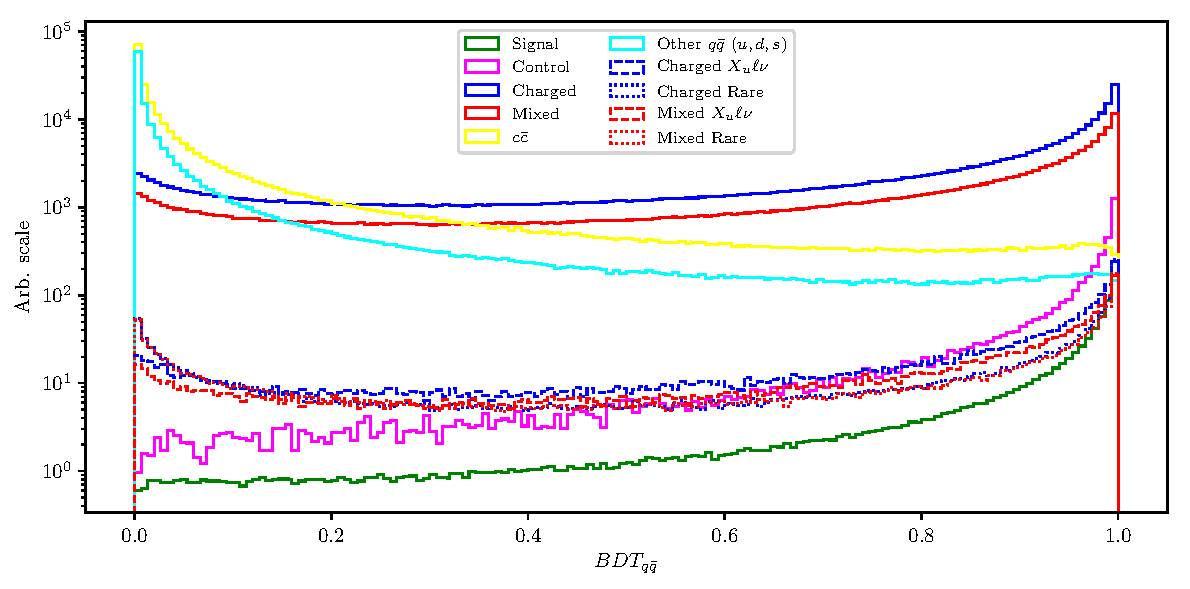
\includegraphics[width=\linewidth]{fig/cs_BDT}
	\caption{Continuum suppression classifier output for signal and various types of background. $B$ candidates from continuum events dominate the lower region, while candidates from $B\bar B$ dominate in the upper region of the classifier output.}
	\label{fig:cs_mva}
\end{figure}

\section{\texorpdfstring{$B\bar B$}{BB-bar} Suppression}

After separating continuum background from $B \bar B$ events, the next step is to train an MVA classifier to recognize our signal candidates among the candidates of other $B \bar B$ background. $B \bar B$ background consists of
\begin{itemize}
	\item $b \to c \ell \nu$ background,
	\item $b \to u \ell \nu$ background,
	\item Other rare decays (radiative, penguin, rare 2- and 3-body decays, \dots).
\end{itemize}

Similarly, the training dataset for this classifier consisted of $2\E5$ candidates, where $50~\%$ of the candidates are correctly reconstructed signal events. The remaining part of the training dataset consists of all background, not including the control sample, because we are not interested in suppressing it directly. The background part of the dataset consists of $75~\%$ charged and neutral $B \bar B$ events in equal proportions, whereas the remaining $25~\%$ is equally populated with charged and neutral $B \bar B$ events from $b \to u \ell \nu$ and other rare decays. The training dataset was proportionally sampled in the same manner as described in section \ref{ss:qqmva}.

In order to separate this kind of background, we must be careful not to introduce correlations with the fit variables ($\Delta E$, $M_{BC}$) or any kind of model dependence (correlation with $q^2$). This means that we can not use any information of the decay particles or the candidate, which is of kinematics nature, such as decay particles momenta, decay angles or other variables with such behavior.

The training variable set consisted of
\begin{itemize}
	\item fit probability of $P(\chi^2,DOF)$ of the signal candidate and the ROE side, separately,
	\item $\cos\theta_{BY}$ from Eq. (\ref{eq:cosby}),
	\item $\cos$ of the angle between momentum and vertex of $X$,\\where $X \in [KK,~KK\ell,~KK\ell\nu]$,
	\item FlavorTagger variables for the two signal-side kaons,
	\item number of kaons, tracks and distant tracks in ROE,
	\item $\theta$ angle of the ROE momentum in CMS frame,
	\item $\xi_Z$ from \cite{PhysRevD.83.032007}
	\item $\Delta z$,
	\item $m_{miss}^2$ from Eq. (\ref{eq:m2def}),
	\item $B \to D^* \ell \nu$ veto variables,
\end{itemize}
where distant tracks are all tracks in ROE which satisfy the condition of $\vert d_0 \vert  > 10.0\e{cm}$ or $\vert z_0 \vert > 20.0\e{cm}$. The last entry, $B \to D^* \ell \nu$ veto variables, are a set of variables where we partially reconstruct the $D^*$ candidate 4-momentum via a linear combination of the $\pi^\pm_s$ 4-momentum in the $D^* \to D \pi_s^\pm$ decay. It helps discard the most dominant $B \to D^* \ell \nu$ background. It is most efficient in the $B^0 \to D^{*-} \ell^+ \nu$ decay, where $D^{*-}$ further decays via $D^{*-} \to \bar D {}^0 \pi^-_s$. Other decays do not contain a charged $\pi_s$ particle and are harder to reconstruct with good precision. This results in larger suppression of the neutral $B \bar B$ background only. Figures \ref{fig:vetoplot} shows the veto variable with a partial reconstruction of a charged $\pi_s^\pm$.

\begin{figure}[H]
	\centering
	\captionsetup{width=0.8\linewidth}
	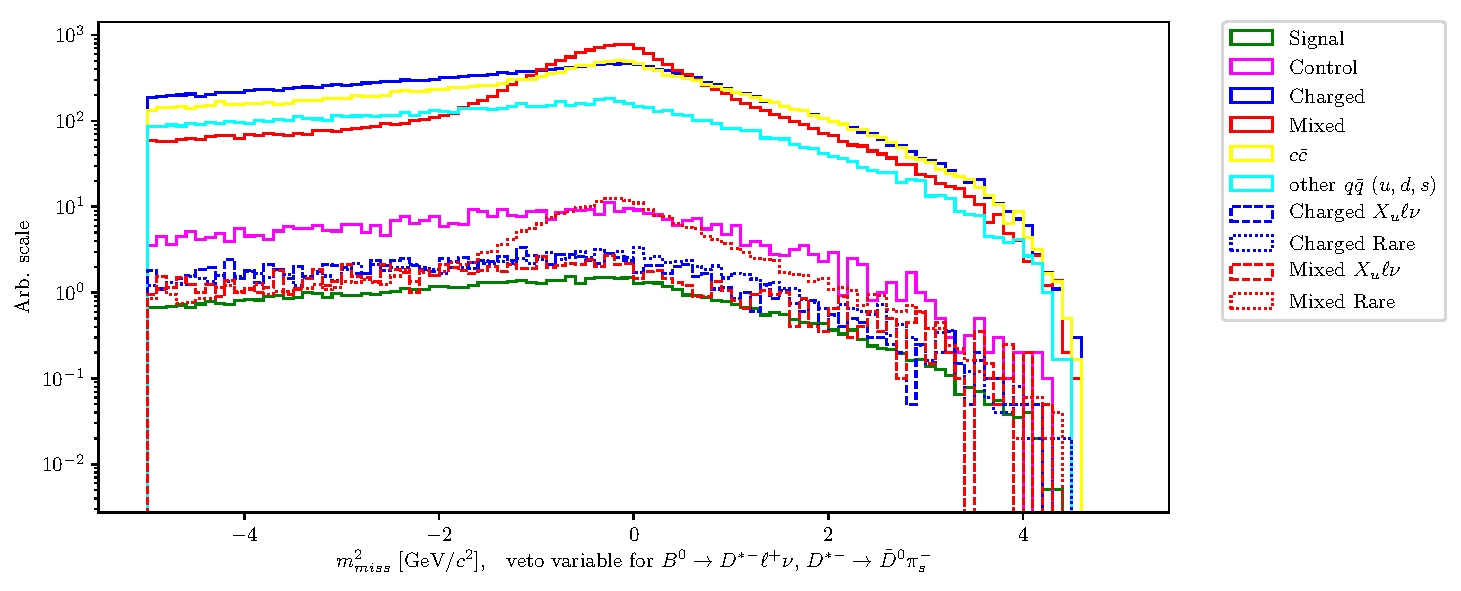
\includegraphics[width=\linewidth]{fig/bb_partial_veto}
	\caption{Distribution of $m_{miss}^2$ for partially reconstructed $B^0 \to D^{*-} \ell^+ \nu$ decays, which serves as a veto.}
	\label{fig:vetoplot}
\end{figure}

When the training is finished and the hyper-parameters of the classifier are optimized, the classifier output, as shown in Figure \ref{fig:bbmva} (left), can be used for background suppression. $B$ meson candidates from $B \bar B$ background are dominant at lower values, while candidates from $B \bar B$ events populate the region with higher values. Since the differences between signal and background $B \bar B$ events are smaller than $B \bar B$ and $q \bar q$ events, the resulting classifier has a smaller separation power than in the previous section.

\subsection{Boosting to Uniformity}
The selection approach with standard classifiers is optimal for counting experiments, as it by construction produces the optimal selection for observing an excess of signal over background events. Today's BDT algorithms, which work in this way, produce non-uniform selection efficiencies and may, as a consequence, shape background distributions to look like signal. In order to minimize such behavior, it is possible to discard variables, which are correlated with the variable of interest (in our case \vars), from the training set. This, however, decreases the classifiers discriminating power. Another approach is to use a novel boosting method, uBoost, which is trained to optimize an integrated $\mathrm{FOM}$ under the constraint that the BDT selection efficiency for the desired class must be uniform. The uBoost algorithm balances the biases to produce the optimal uniform selection \cite{stevens2013uboost}.

The training set used in this training is the same as described at the beginning of this chapter, along with the same set of training variables. It will be seen later that the standard BDT classifier shapes the background to look like signal mostly in the $M_{BC}$ picture, therefore we train the uBDT classifier with a uniformity constraint in the $M_{BC}$ variable for background candidates with the uBoost algorithm. The resulting classifier output is shown in Figure \ref{fig:bbmva} (right). For this classifier, the separation power between signal and background seems worse, however, the shapes of backgrounds differ significantly, which greatly affects the performance of signal extraction.

\begin{figure}[H]
	\centering
	\captionsetup{width=0.8\linewidth}
	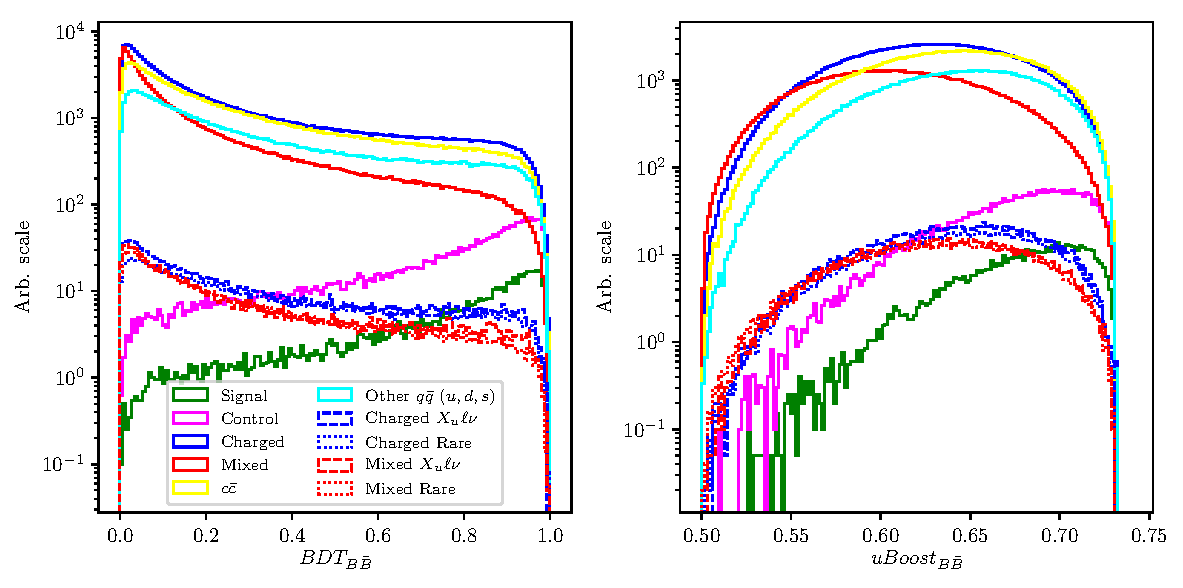
\includegraphics[width=\linewidth]{fig/bb_BDT}
	\caption{$B\bar B$ suppression classifier output for signal and various types of background for the standard BDT classifier (left) and the uBDT classifier (right). $B$ candidates from $B\bar B$ background events dominate the lower region, while signal and control candidates dominate in the upper region of the classifier output.}
	\label{fig:bbmva}
\end{figure}

\section{Selection Optimization}\label{sec:selection-optimization}

Instead of two separate $q \bar q$ and $B \bar B$ $\mathrm{FOM}$ optimizations, it is more efficient to do a simultaneous 2D $\mathrm{FOM}$ optimization, since the two classifiers are not completely uncorrelated. In the same manner, as before, $\mathrm{FOM}$ is optimized for perfectly reconstructed signal candidates in the signal window, after all the pre-cuts, signal categorization, and after cutting out the background resonances and the control decay. The $\mathrm{FOM}$ plot with the optimal point for both $B \bar B$ MVA classifiers is shown in Figure \ref{fig:mvafom}.

\begin{figure}[H]
	\centering
	\captionsetup{width=0.8\linewidth}
	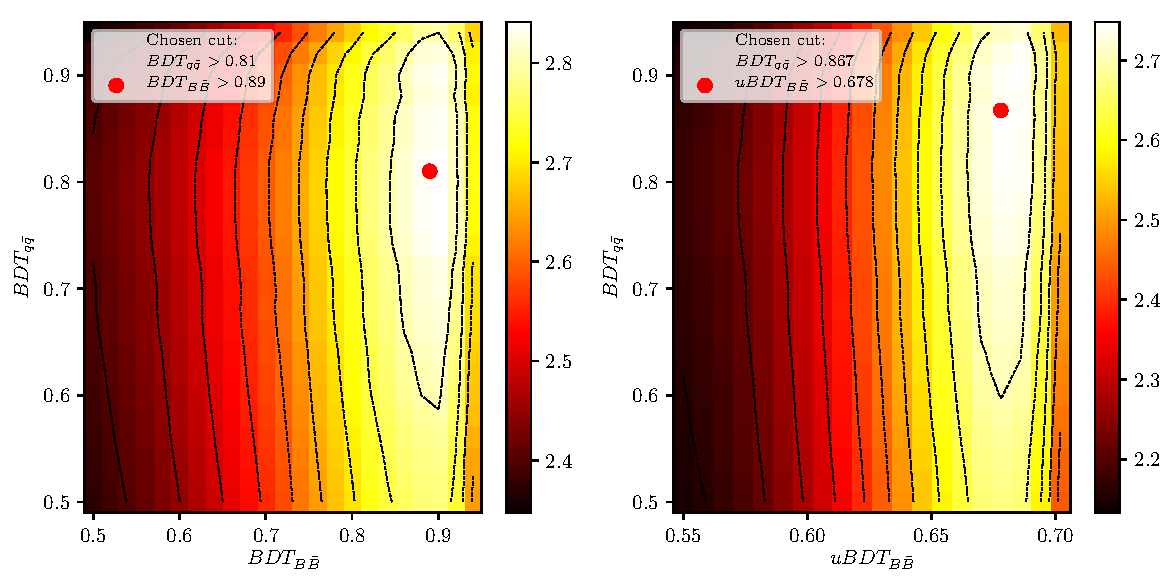
\includegraphics[width=\linewidth]{fig/mva_fom}
	\caption{2D $\mathrm{FOM}$ optimization of continuum suppression classifier and the standard BDT (left) and uBDT (right) $B\bar B$ suppression classifier.}
	\label{fig:mvafom}
\end{figure}

We can compare signal and major background distributions of \vars~after the 2D $\mathrm{FOM}$ optimization for both classifiers. Figure \ref{fig:opt01c} shows the arbitrary (left) and normalized scale (right) for $\Delta E$ (top) and $M_{BC}$ (bottom) for the final sample optimized with the standard BDT classifier, while Figure \ref{fig:opt1dc} shows similarly for the final sample optimized with uBDT classifier. We can see that there is considerably more background in the latter case, however, also shapes of background and signal distributions differ greatly, meaning there is less room for correlation. The biggest change seems to be in the shape of the $M_{BC}$ distribution, where the background component is much more signal like in the final sample optimized with the standard BDT classifier than in the other case.  Additionally, the shapes are more easily constrained in the latter case, since they are present in regions where no signal is expected. The total numbers of expected signal candidates and the signal-to-noise ratios for both classifiers are:
\begin{itemize}
	\item Standard BDT: $N_{sig} = 176,\quad N_{sig}/N_{bkg} = 4.83~\%$,
	\item uBDT: $N_{sig} = 264,\quad N_{sig}/N_{bkg} = 1.33~\%$.
\end{itemize}
Due to the large difference in \vars~shape, we will continue the analysis with the uBDT classifier, although the comparison between both methods will be shown for the final fit result in the next chapter.

\begin{figure}[H]
	\centering
	\captionsetup{width=0.8\linewidth}
	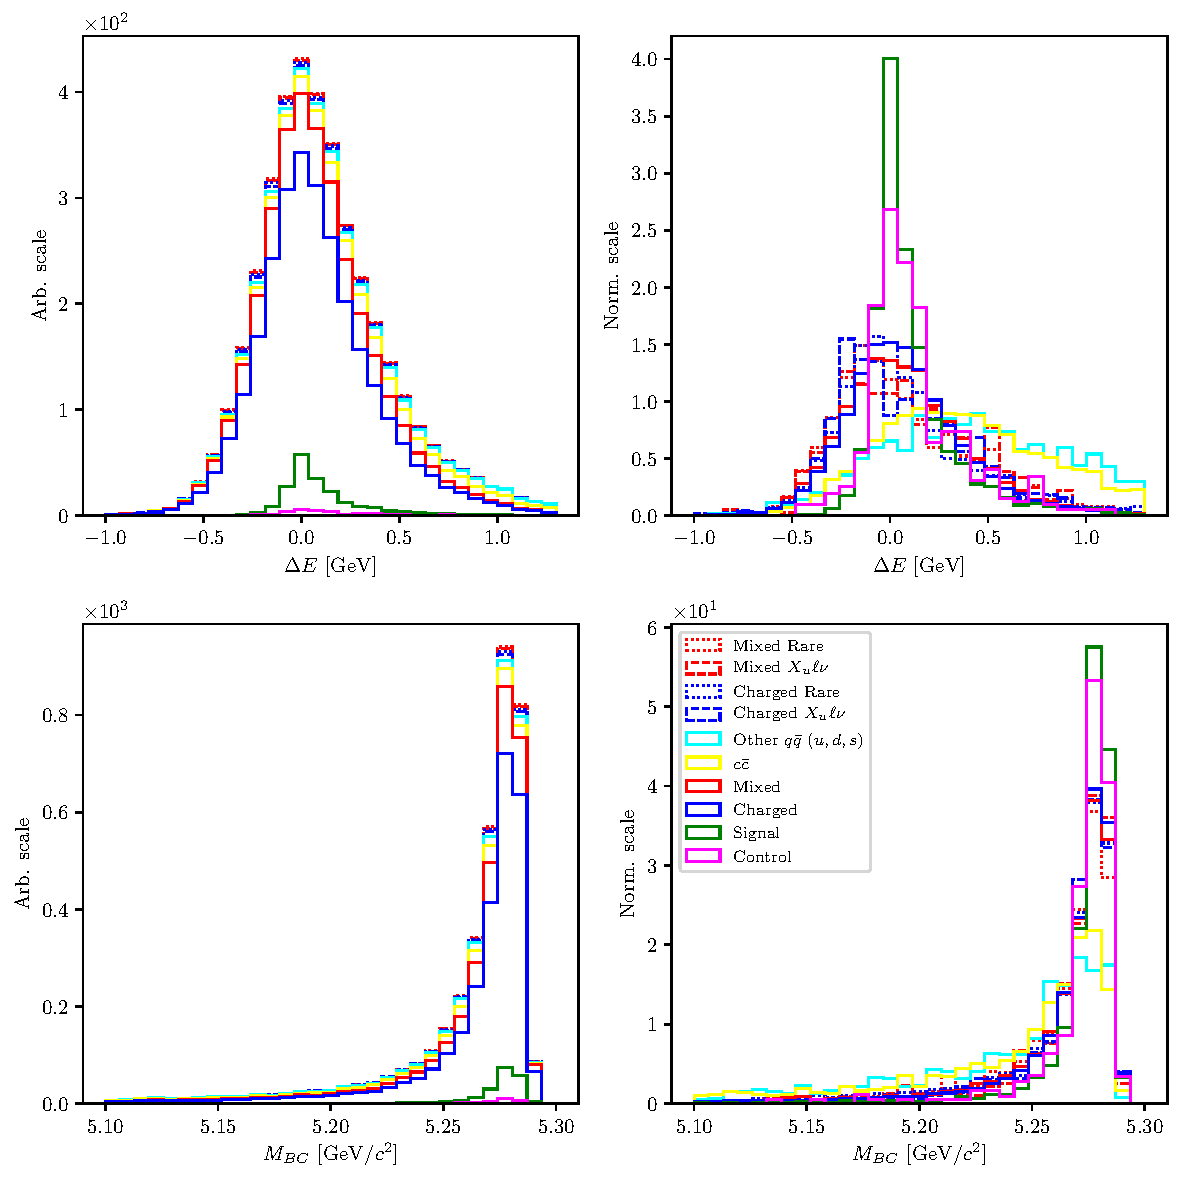
\includegraphics[width=\linewidth]{fig/opt_BB}
	\caption{Arbitrary (left) and normalized scale (right) for $\Delta E$ (top) and $M_{BC}$ (bottom) for the final sample optimized with the standard BDT classifier.}
	\label{fig:opt01c}
\end{figure} 

\begin{figure}[H]
	\centering
	\captionsetup{width=0.8\linewidth}
	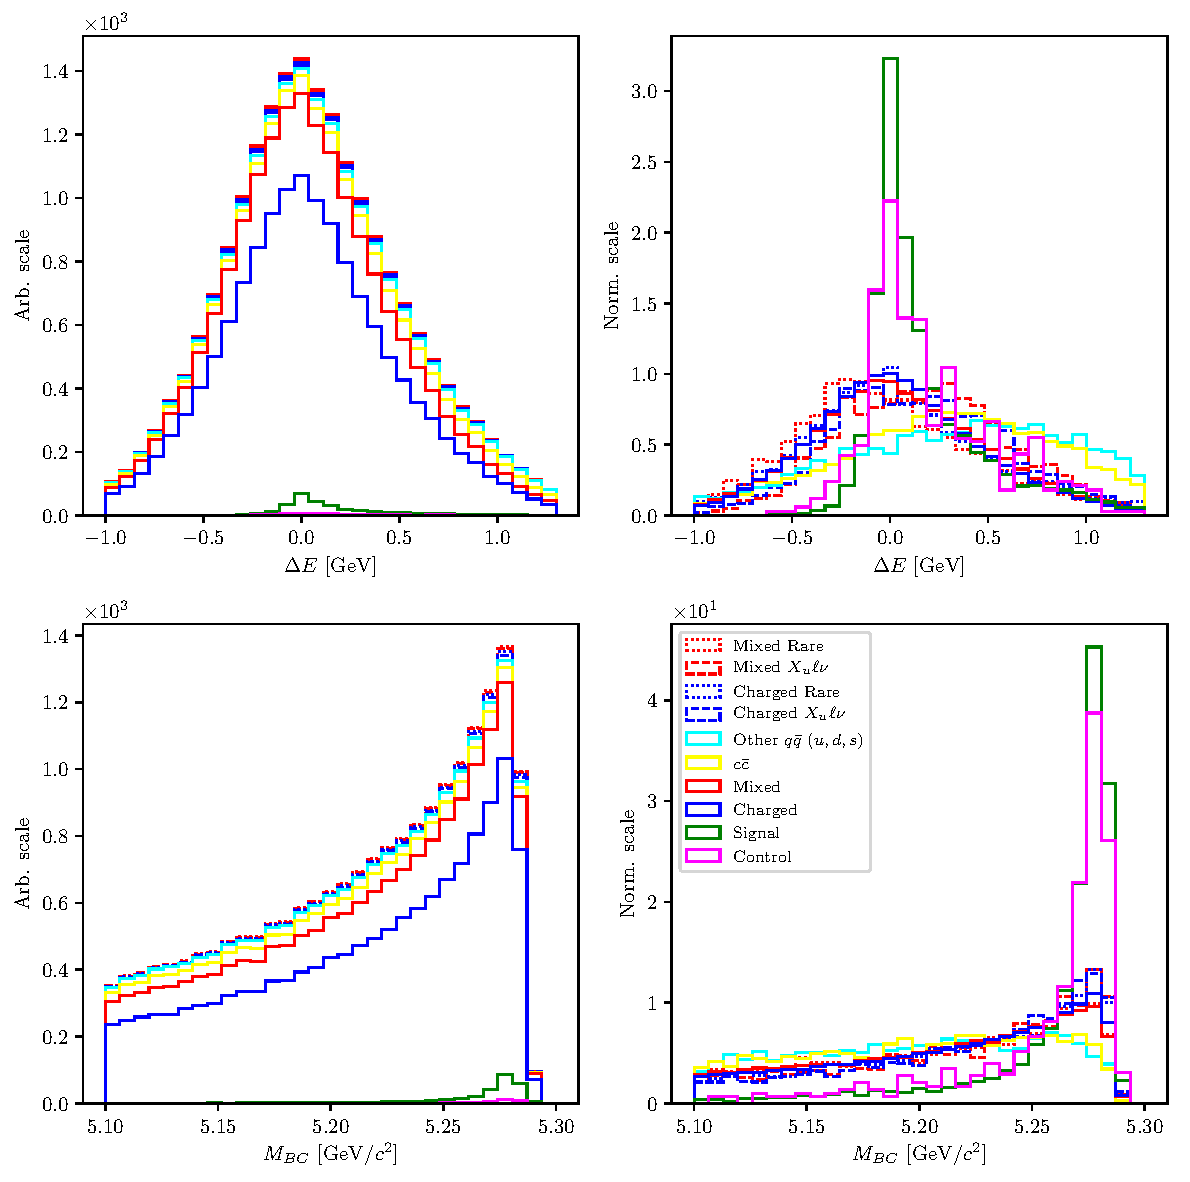
\includegraphics[width=\linewidth]{fig/opt_uBB}
	\caption{Arbitrary (left) and normalized scale (right) for $\Delta E$ (top) and $M_{BC}$ (bottom) for the final sample optimized with the uBDT classifier for $B \bar B$ suppression.}
	\label{fig:opt1dc}
\end{figure} 

\subsection{\texorpdfstring{$B \bar B$}{BB-bar} Background Composition and Lepton Veto}

The majority of background candidates after the final selection is represented by candidates from $B \bar B$ events. In order to suppress this background even further, we need to take a look at its structure and recognize various contributions to this part of the background. Figure \ref{fig:sig_bkg_all_before} shows \vars~for the most significant contributions, along with $m_{KK}$. While most of the candidates come from events where all reconstructed charged particles in the signal decay do not come from one $B$ meson, but both of them, these candidates are not so problematic, because their distribution is rather smooth and frequent in regions where we expect no signal. On the other hand, there are also contributions from $B$ meson decays which produce more signal-like distributions. We will denote the first kind of background as $\Upsilon(4S)$-matched and the second kind as the $B$-matched $B \bar B$ background. Fortunately, these decays are well known and well measured, so their yields can be constrained. Especially problematic is the double semileptonic decay $B \to \bar D {}^{(*)} \ell^+ \nu,~D^+ \to \bar K^- \ell^+ \nu$, where the secondary lepton is misidentified as a kaon. Even though the decay has two neutrinos, these events survive the $m_{miss}^2$ selection cut and produce peaks at the same positions as signal distributions, while exhibiting only a slightly worse resolution. 

\begin{figure}[H]
	\centering
	\captionsetup{width=0.8\linewidth}
	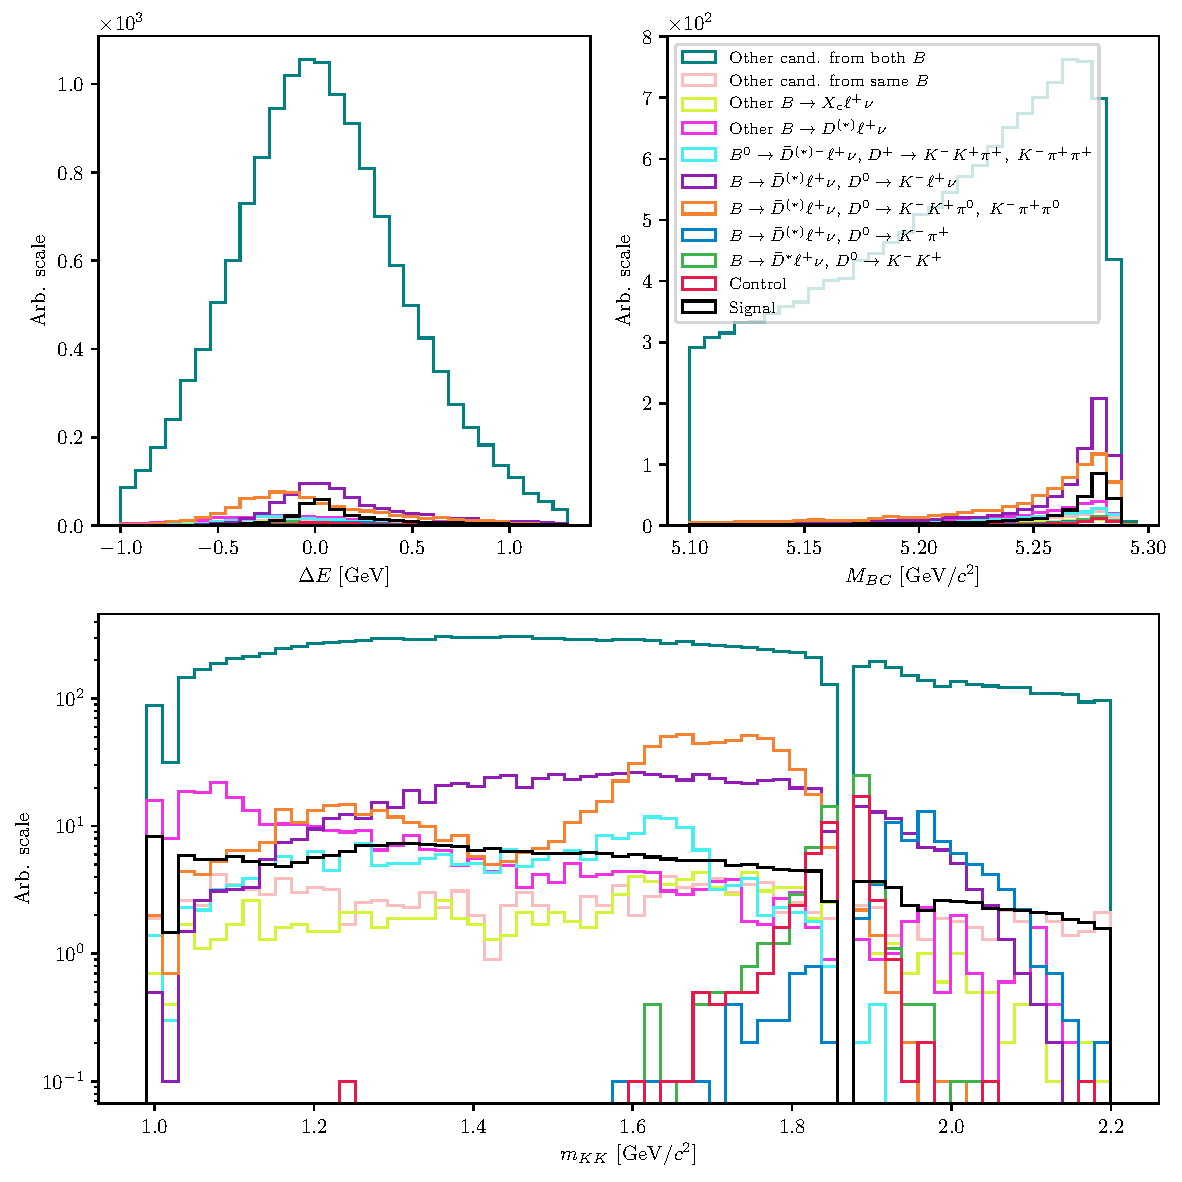
\includegraphics[width=\linewidth]{fig/sig_BKG_composition_all_before.pdf}
	\caption{$\Delta E$ (left), $M_{BC}$ (right) and $m_{KK}$ (bottom) for major contributions to the $B \bar B$ background in the signal cut region. $\Upsilon(4S)$-matched backgrounds represents the majority, but has a smooth and wide background, which has a distinguishable shape from signal. $B$-matched contributions show a peak in $M_{BC}$ and sometimes in $\Delta E$, but can be constrained using existing measurements.}
	\label{fig:sig_bkg_all_before}
\end{figure} 

In order to suppress these candidates, a lepton veto can be applied to both kaons, stating that neither of the kaons should exhibit lepton-like properties. On the candidates passing the final selection, we optimize the $eID$ and $\mu ID$ PID cuts, where $S$ and $B$ in Eq. \ref{eq:fom} are represented by perfect signal candidates and by background candidates, respectively, whereas in the latter case a lepton has been misidentified as a kaon. 2D FOM plots for both kaons are shown in Figure \ref{fig:lepVeto}, where it can be seen that in the majority of the cases, an electron is misidentified as the kaon with the opposite charge to the $B$ meson. With the optimal cuts of 
\begin{itemize}
	\item $K_0:~eID < 0.8,$
	\item $K_1:~eID < 0.1,~\mu ID < 0.8,$
\end{itemize}
we reject $77.5\%$ of candidates from the double semileptonic decays, while efficiency loss of signal and other types of $B \bar B$ background is about $5-6\%$. The $B \bar B$ background after the lepton veto cuts is shown in Figure \ref{fig:sig_bkg_all_after} for the signal cut region, and in Figure \ref{fig:cs_bkg_after} for the control cut region.

\begin{figure}[H]
	\centering
	\captionsetup{width=0.8\linewidth}
	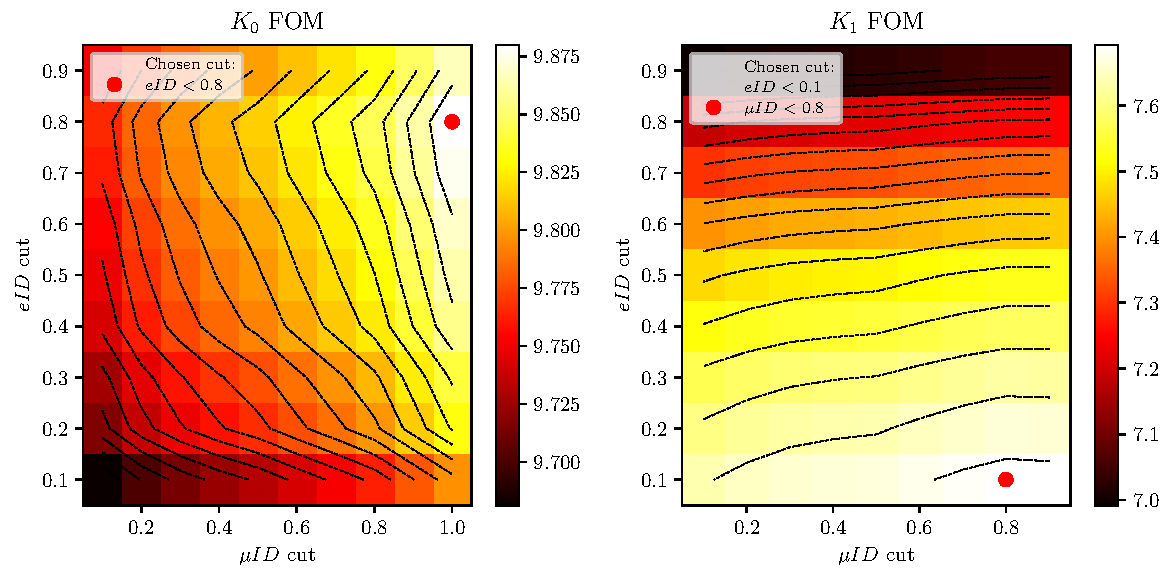
\includegraphics[width=\linewidth]{fig/lepVeto}
	\caption{2D FOM for optimal $eID$ and $\mu ID$ cuts on same-sign (left) and opposite-sign (right) kaons with respect to the $B$ meson charge. For double semileptonic background component, in most cases an electron is missidentified as the opposite-sign kaon in the reconstruction chain.}
	\label{fig:lepVeto}
\end{figure} 

\begin{figure}[H]
	\centering
	\captionsetup{width=0.8\linewidth}
	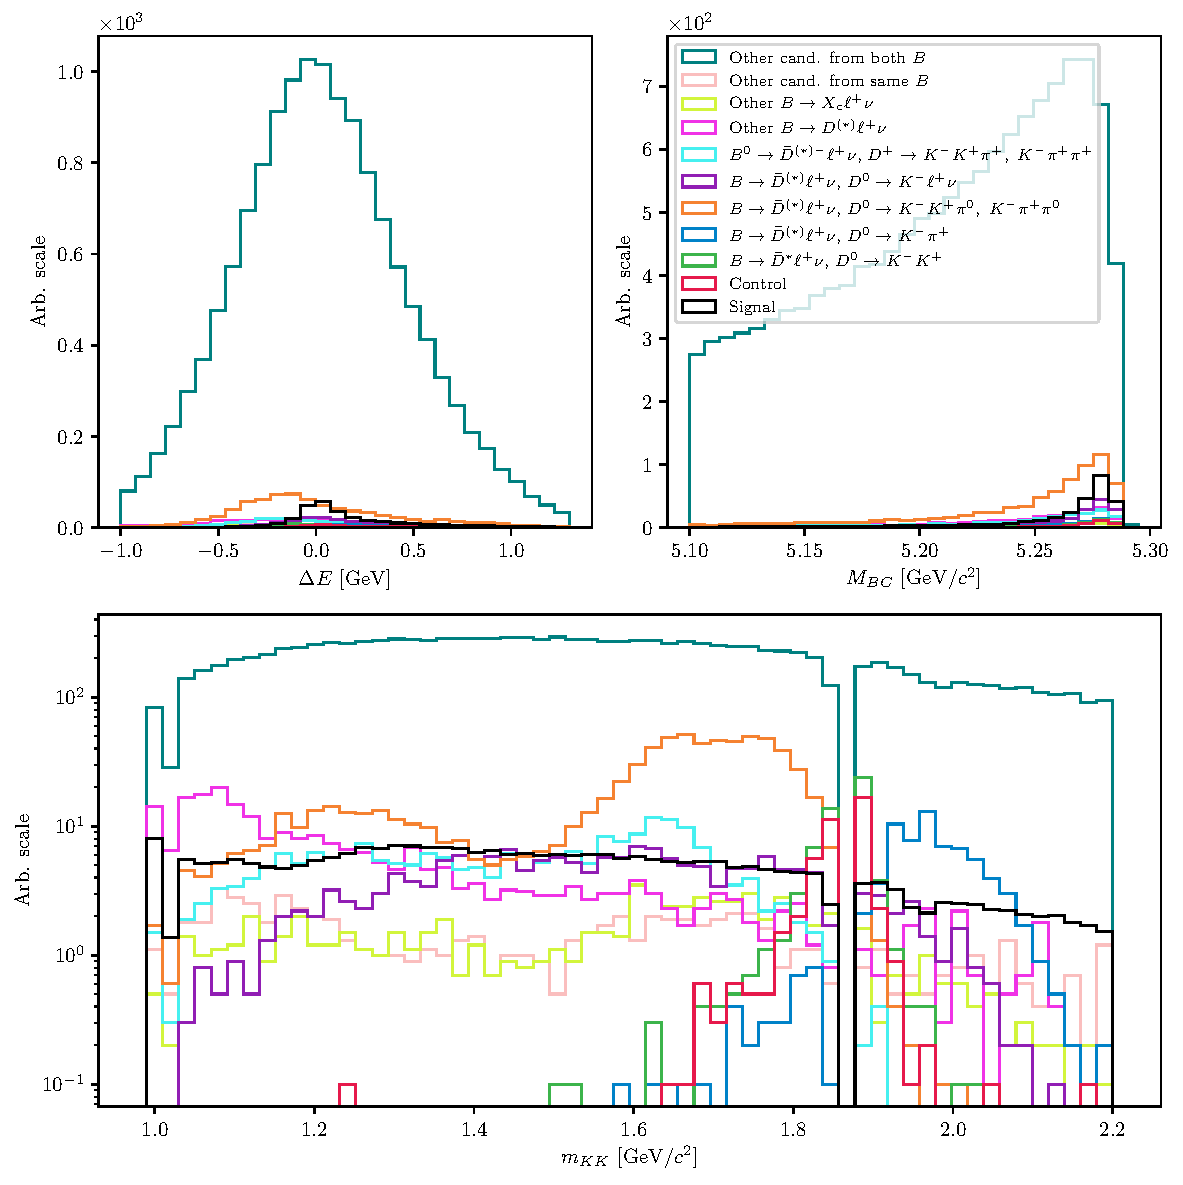
\includegraphics[width=\linewidth]{fig/sig_BKG_composition_all_after}
	\caption{$\Delta E$ (left), $M_{BC}$ (right) and $m_{KK}$ (bottom) for major contributions to the $B \bar B$ background in the signal cut region after the lepton veto. The double semileptonic background component is suppressed by a factor of $4-5$.}
	\label{fig:sig_bkg_all_after}
\end{figure} 

\begin{figure}[H]
	\centering
	\captionsetup{width=0.8\linewidth}
	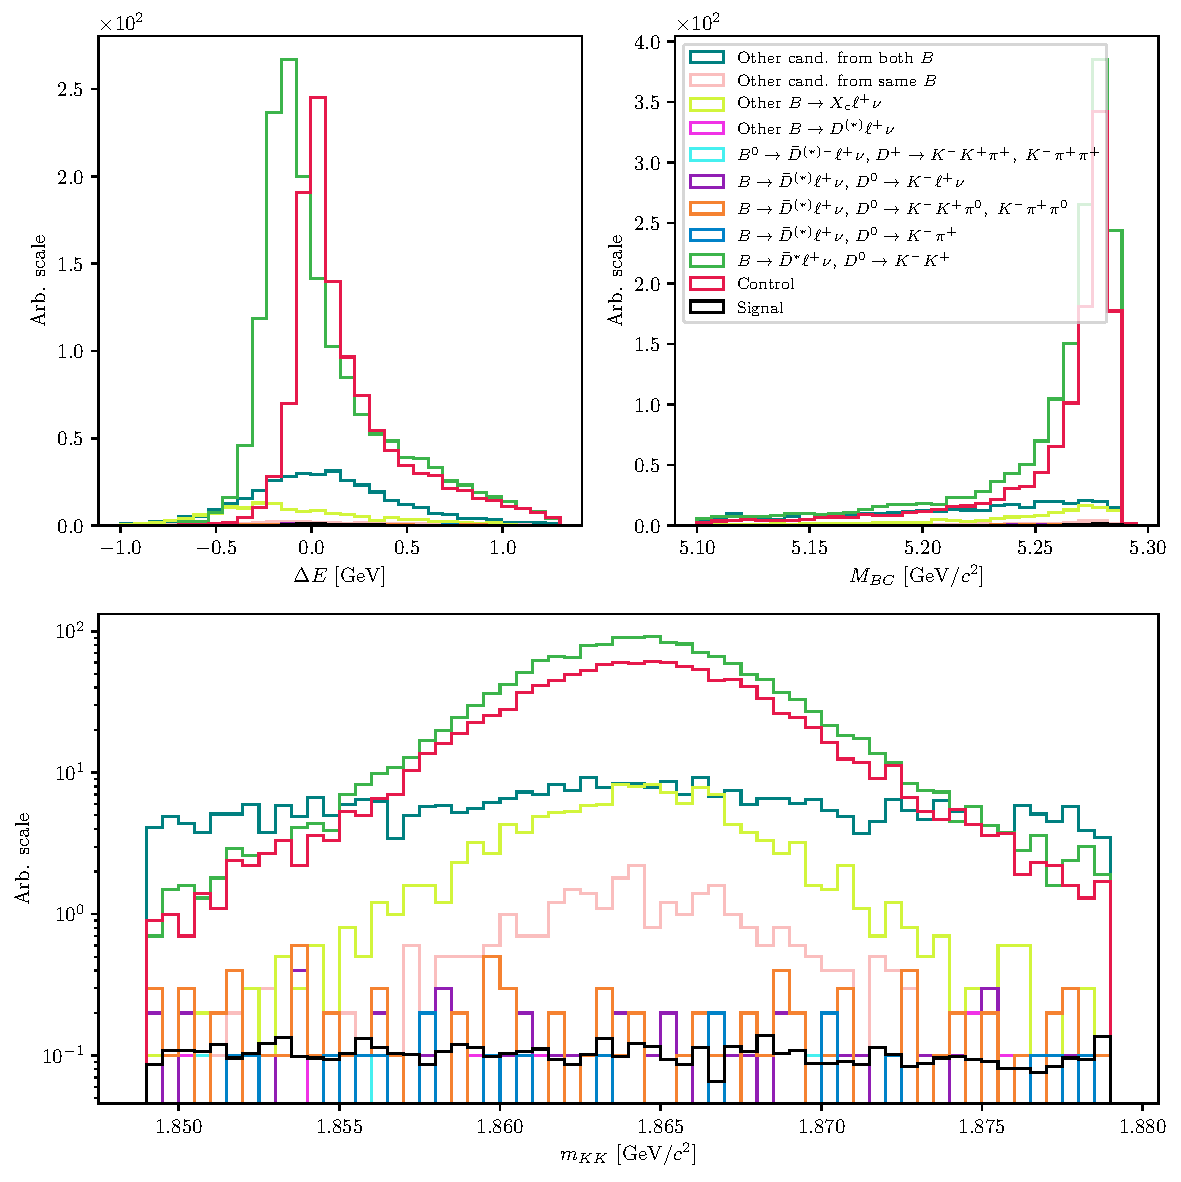
\includegraphics[width=\linewidth]{fig/cs_BKG_composition_after}
	\caption{$\Delta E$ (left), $M_{BC}$ (right) and $m_{KK}$ (bottom) for major contributions to the $B \bar B$ background in the control cut region after the lepton veto. The major component in this case are other $B \to D^* \ell+ \nu,~D \to K^+K^-$ decays, besides the control decay.}
	\label{fig:cs_bkg_after}
\end{figure} 

\section{Data and MC Agreement}

With the final selection in place, we can check the data and MC agreement by checking the control decay region in on- and off- resonance data. Off-resonance samples provide the ability to check the agreement of the $q\bar q$ background component, while on-resonance samples can be used to check the validity of the control MC sample and, consequentially, the signal MC sample.

\subsection{Off-resonance Data}

The off-resonance data were collected at $60\e{MeV}$ below the $\Upsilon(4S)$ resonance peak energy in order to determine the non-$B\bar B$ background. It, therefore, offers a direct view of the $q\bar q$ background data sample, which we can compare to the off-resonance MC sample. Figure \ref{fig:offres_control} shows $\Delta E$, $M_{BC}$ and the $q \bar q$ classifier output, $BDT_{q\bar q}$, for off-resonance data and stacked MC in the control region, before any MVA cuts, where the MC sample was scaled down by a factor of $6$, due to 6 streams of MC. These figures do not show a fit to data, but merely an overlay of data and stacked MC distributions, and show good data and MC agreement of the off-resonance sample already before the fit. More importantly than the normalization, the shape of data and MC also seems to be the same, so further corrections of \vars~on MC are not necessary. This is also consistent by the flatness of the ratio function for \vars, shown in the same Figure. There seems to be a difference in the classifier performance for the continuum background suppression on data and MC. This leads to further differences between data and MC in the $q \bar q$ sample after the classifier cut, but we estimate that these differences are negligible, since a relatively small amount of continuum background passes the selection, compared to other background types.
\begin{figure}[H]
	\centering
	\captionsetup{width=0.8\linewidth}
	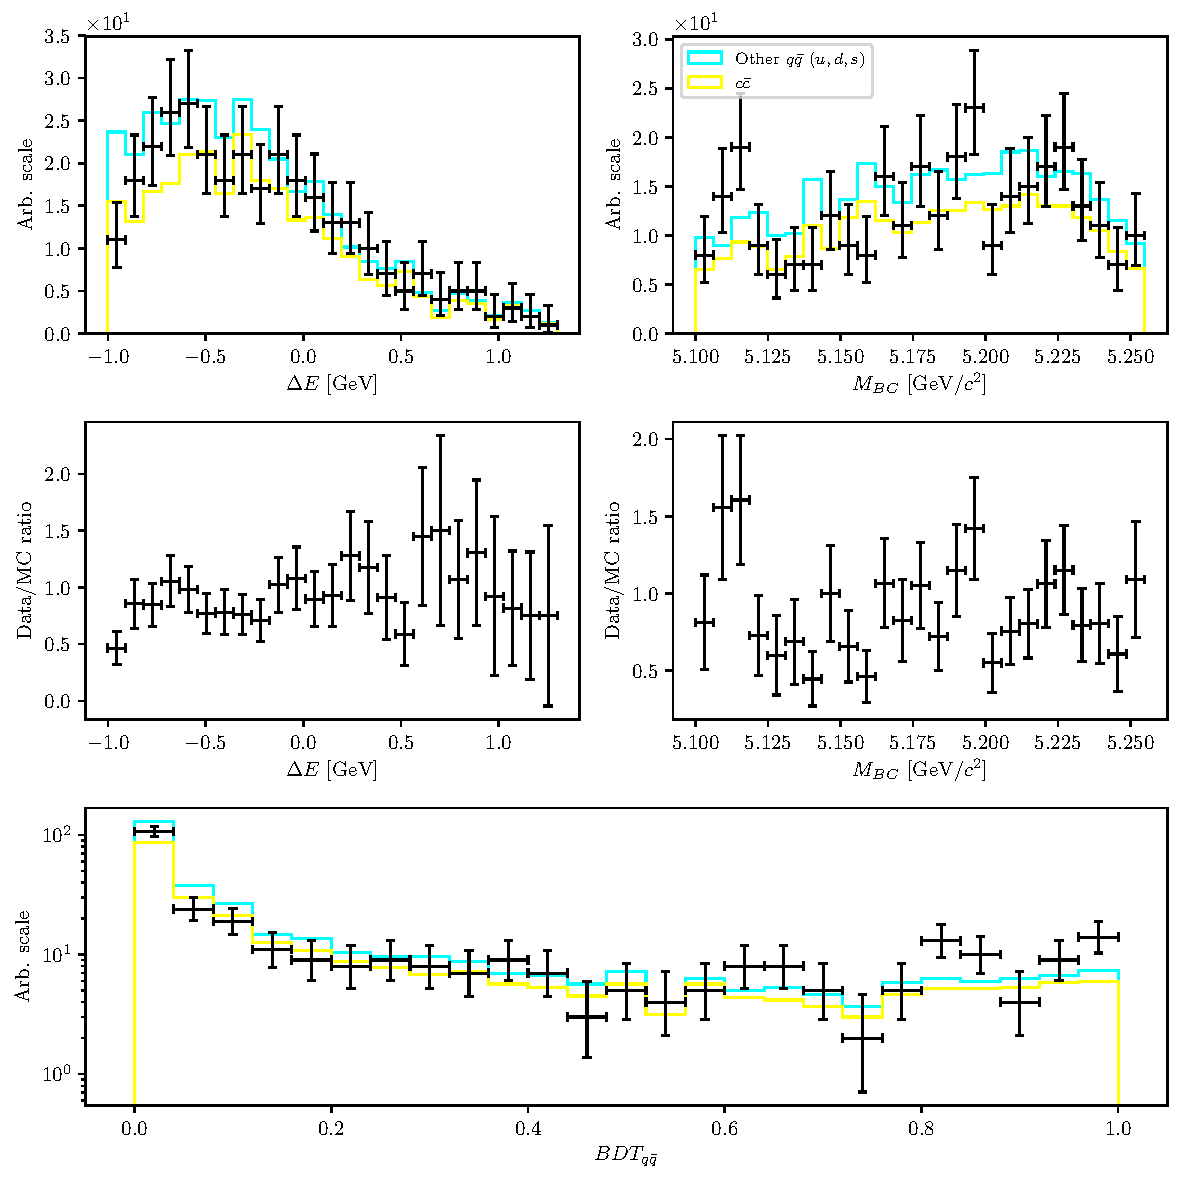
\includegraphics[width=\linewidth]{fig/offres_control}
	\caption{$\Delta E$ (left), $M_{BC}$ (right) and the $q \bar q$ classifier output (bottom), for off-resonance data and MC in the control region before any MVA cuts.}
	\label{fig:offres_control}
\end{figure}

\subsection{On-resonance Data}

We can repeat the check on on-resonance data. Figure \ref{fig:onres_control} shows $\Delta E$, $M_{BC}$ and $BDT_{q \bar q}$, where one can see inconsistencies between data and stacked MC on the lower spectrum, where continuum background is dominant. These figures again do not show the fit, but merely an overlay of data to the stacked MC distributions, where we see that the MC is over-estimated in the lower region of the continuum suppression MVA output, most likely due to additional disagreements from other sources. On the other hand, data and MC seem to agree well in the upper part of the spectrum, where $B \bar B$ events are dominant. Overall, data and MC seem to agree well already off-the-shelf after all the pre-cuts and without any corrections. This means that the modeling of this MC sample is very precise in this particular region of data and that there are no significant differences between data an MC for the control sample and the signal sample.
\begin{figure}[H]
	\centering
	\captionsetup{width=0.8\linewidth}
	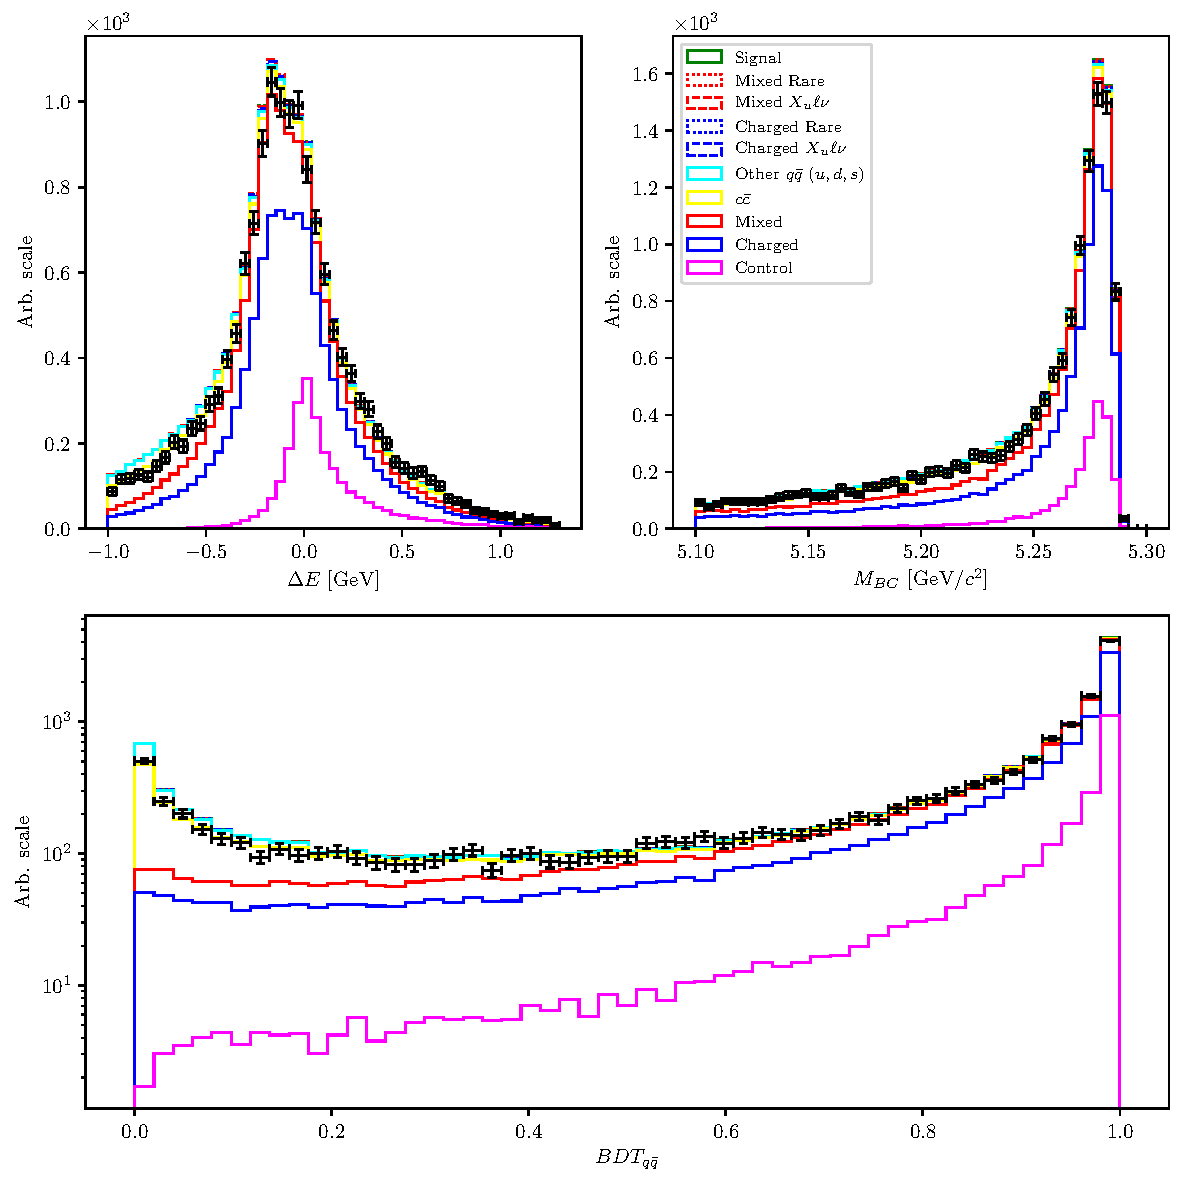
\includegraphics[width=\linewidth]{fig/onres_control}
	\caption{$\Delta E$ (left), $M_{BC}$ (right) and the $q \bar q$ classifier output (bottom), for on-resonance data and MC in the control region before any MVA cuts.}
	\label{fig:onres_control}
\end{figure}